% úvod
Domácí brána je v podstatě velmi jednoduchý program, který pouze přeposílá data, jež obdrží od NATS serveru, do 
\gls{firebase} Firestoru. Z důvodů popsaných výše jsem, jako jazyk opět zvolil \gls{go}.

% graf
\begin{figure}[H]
    \centering
    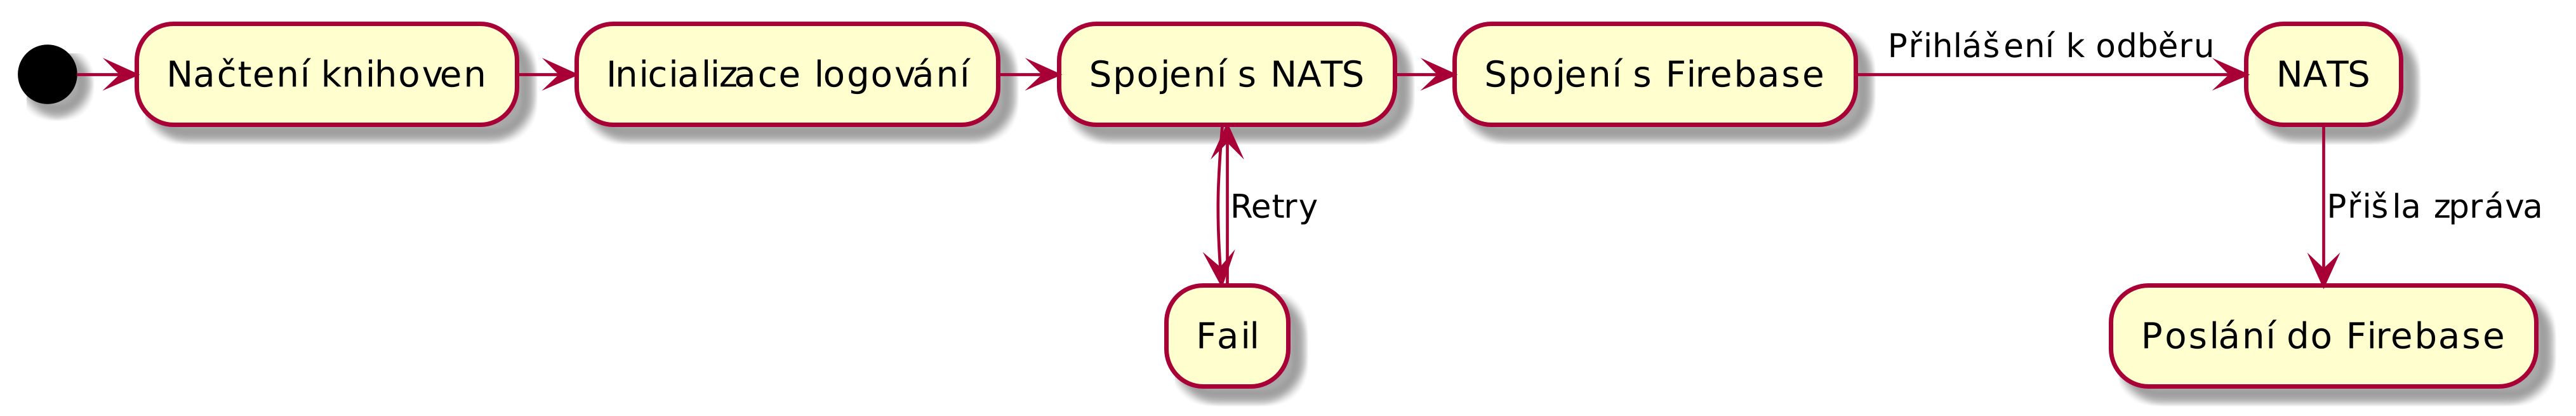
\includegraphics[width=\textwidth]{gateway.png}
    \caption{Průběh programu}
\end{figure}

% sběr informací
Spojení s NATSem je stejné, jako u odesílání dat. Jediný rozdíl je v aplikační části, kdy data neodesílám, ale přijímám. 
Příjem probíhá tak, že se přihlásím k odběru kanálu, do kterého měřící stanice odesílá data a pro každou zprávu, která 
přijde spustím funkci, která ji pošle dál. Trochu nestandardní je přihlášení k odběru. Používám takzvanou \uv{durable 
subscription}. Jedná se o funkci NATS streaming serveru, která mi umožňuje přihlásit se pod určitým jménem a server si 
pak pamatuje, jakou poslední zprávu mi posílal, takže když dojde k výpadku, po opětovném připojení mi pošle všechny 
zprávy, které jsem dosud nedostal \parencite{root.cz:NATS-streaming}.

% odesílání do cloudu
Jediné co funkce zpracovávající naměřená data dělá, je přeposílání do cloudu. Celou komunikaci s cloudem jsem v podstatě 
opsal z dokumentace firestoru (\url{https://firebase.google.com/docs/firestore}). Začíná to inicializací spojení, 
přihlašování probíhá přes vygenerovaný soubor s privátním klíčem. Soubor jsem pouze stáhnul, uložil někam, kde k němu má 
aplikace přístup a řekl jsem jí kde ho má hledat. O zbytek se postará Googlem poskytovaná \gls{knihovna}. To proběhne po 
startu programu, a pak se vytvořené spojení používá až do konce. Poté už se jen přeposílají data.

% krok 1
\begin{figure}[H]
    \centering
    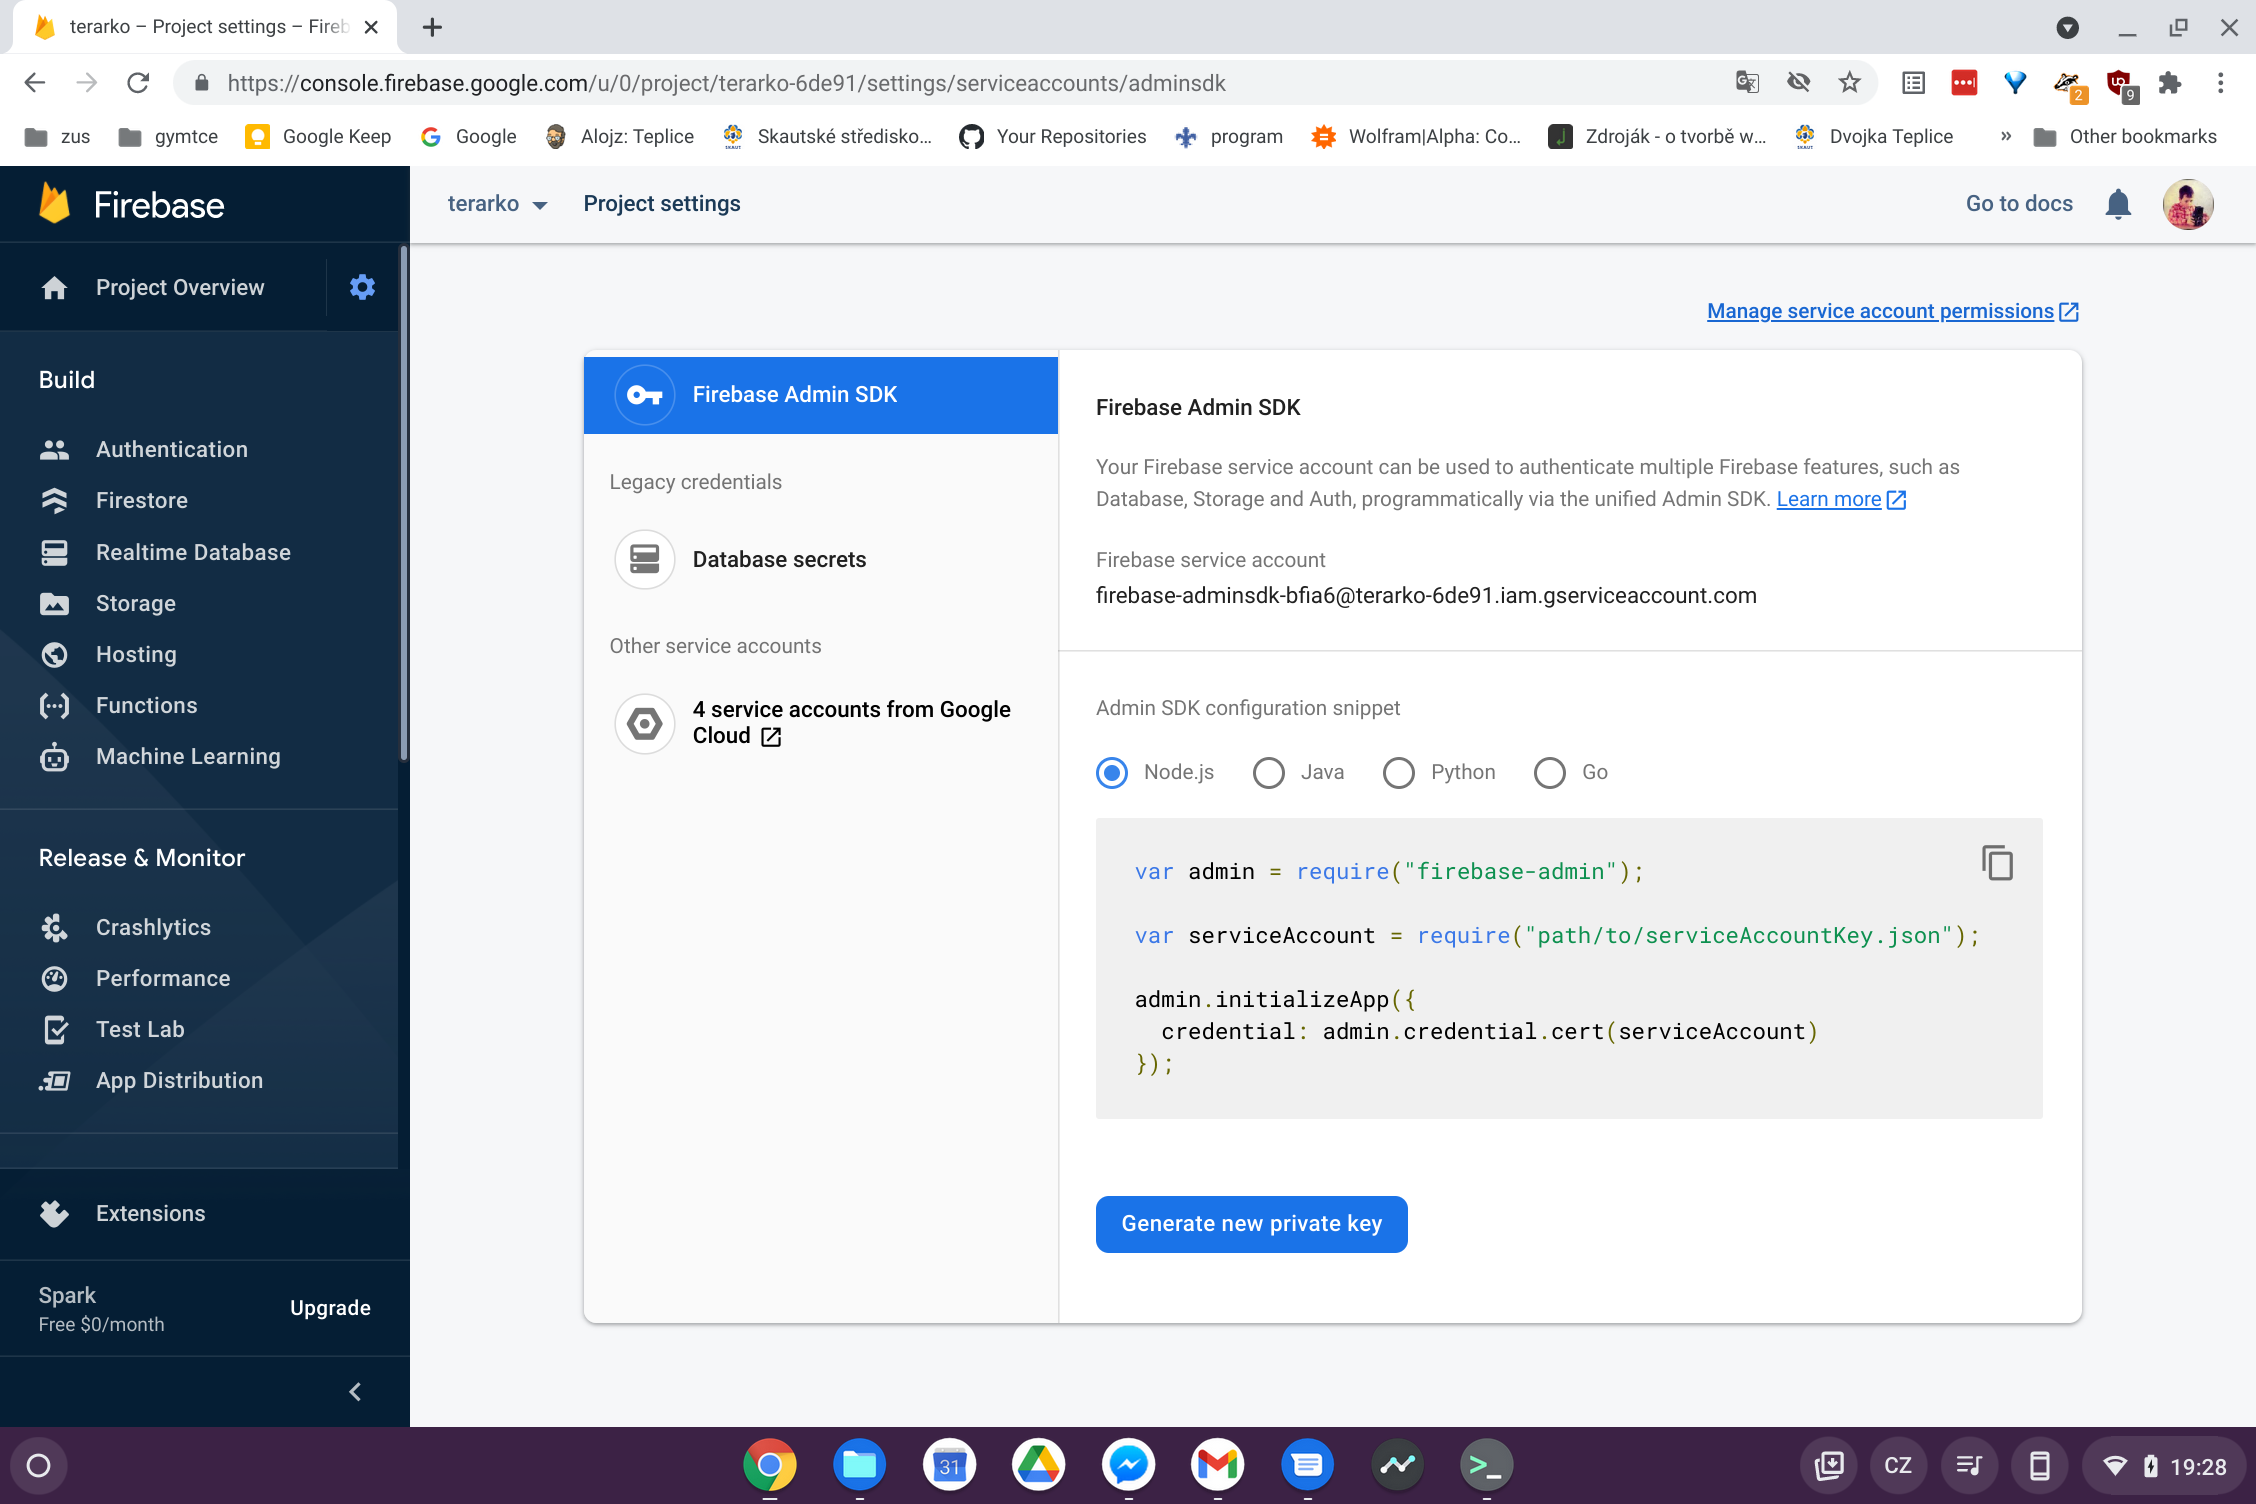
\includegraphics[width=0.8\textwidth]{key1.png}
    \caption{Vygenerování klíče, krok 1}
\end{figure}
% krok 2
\begin{figure}[H]
    \centering
    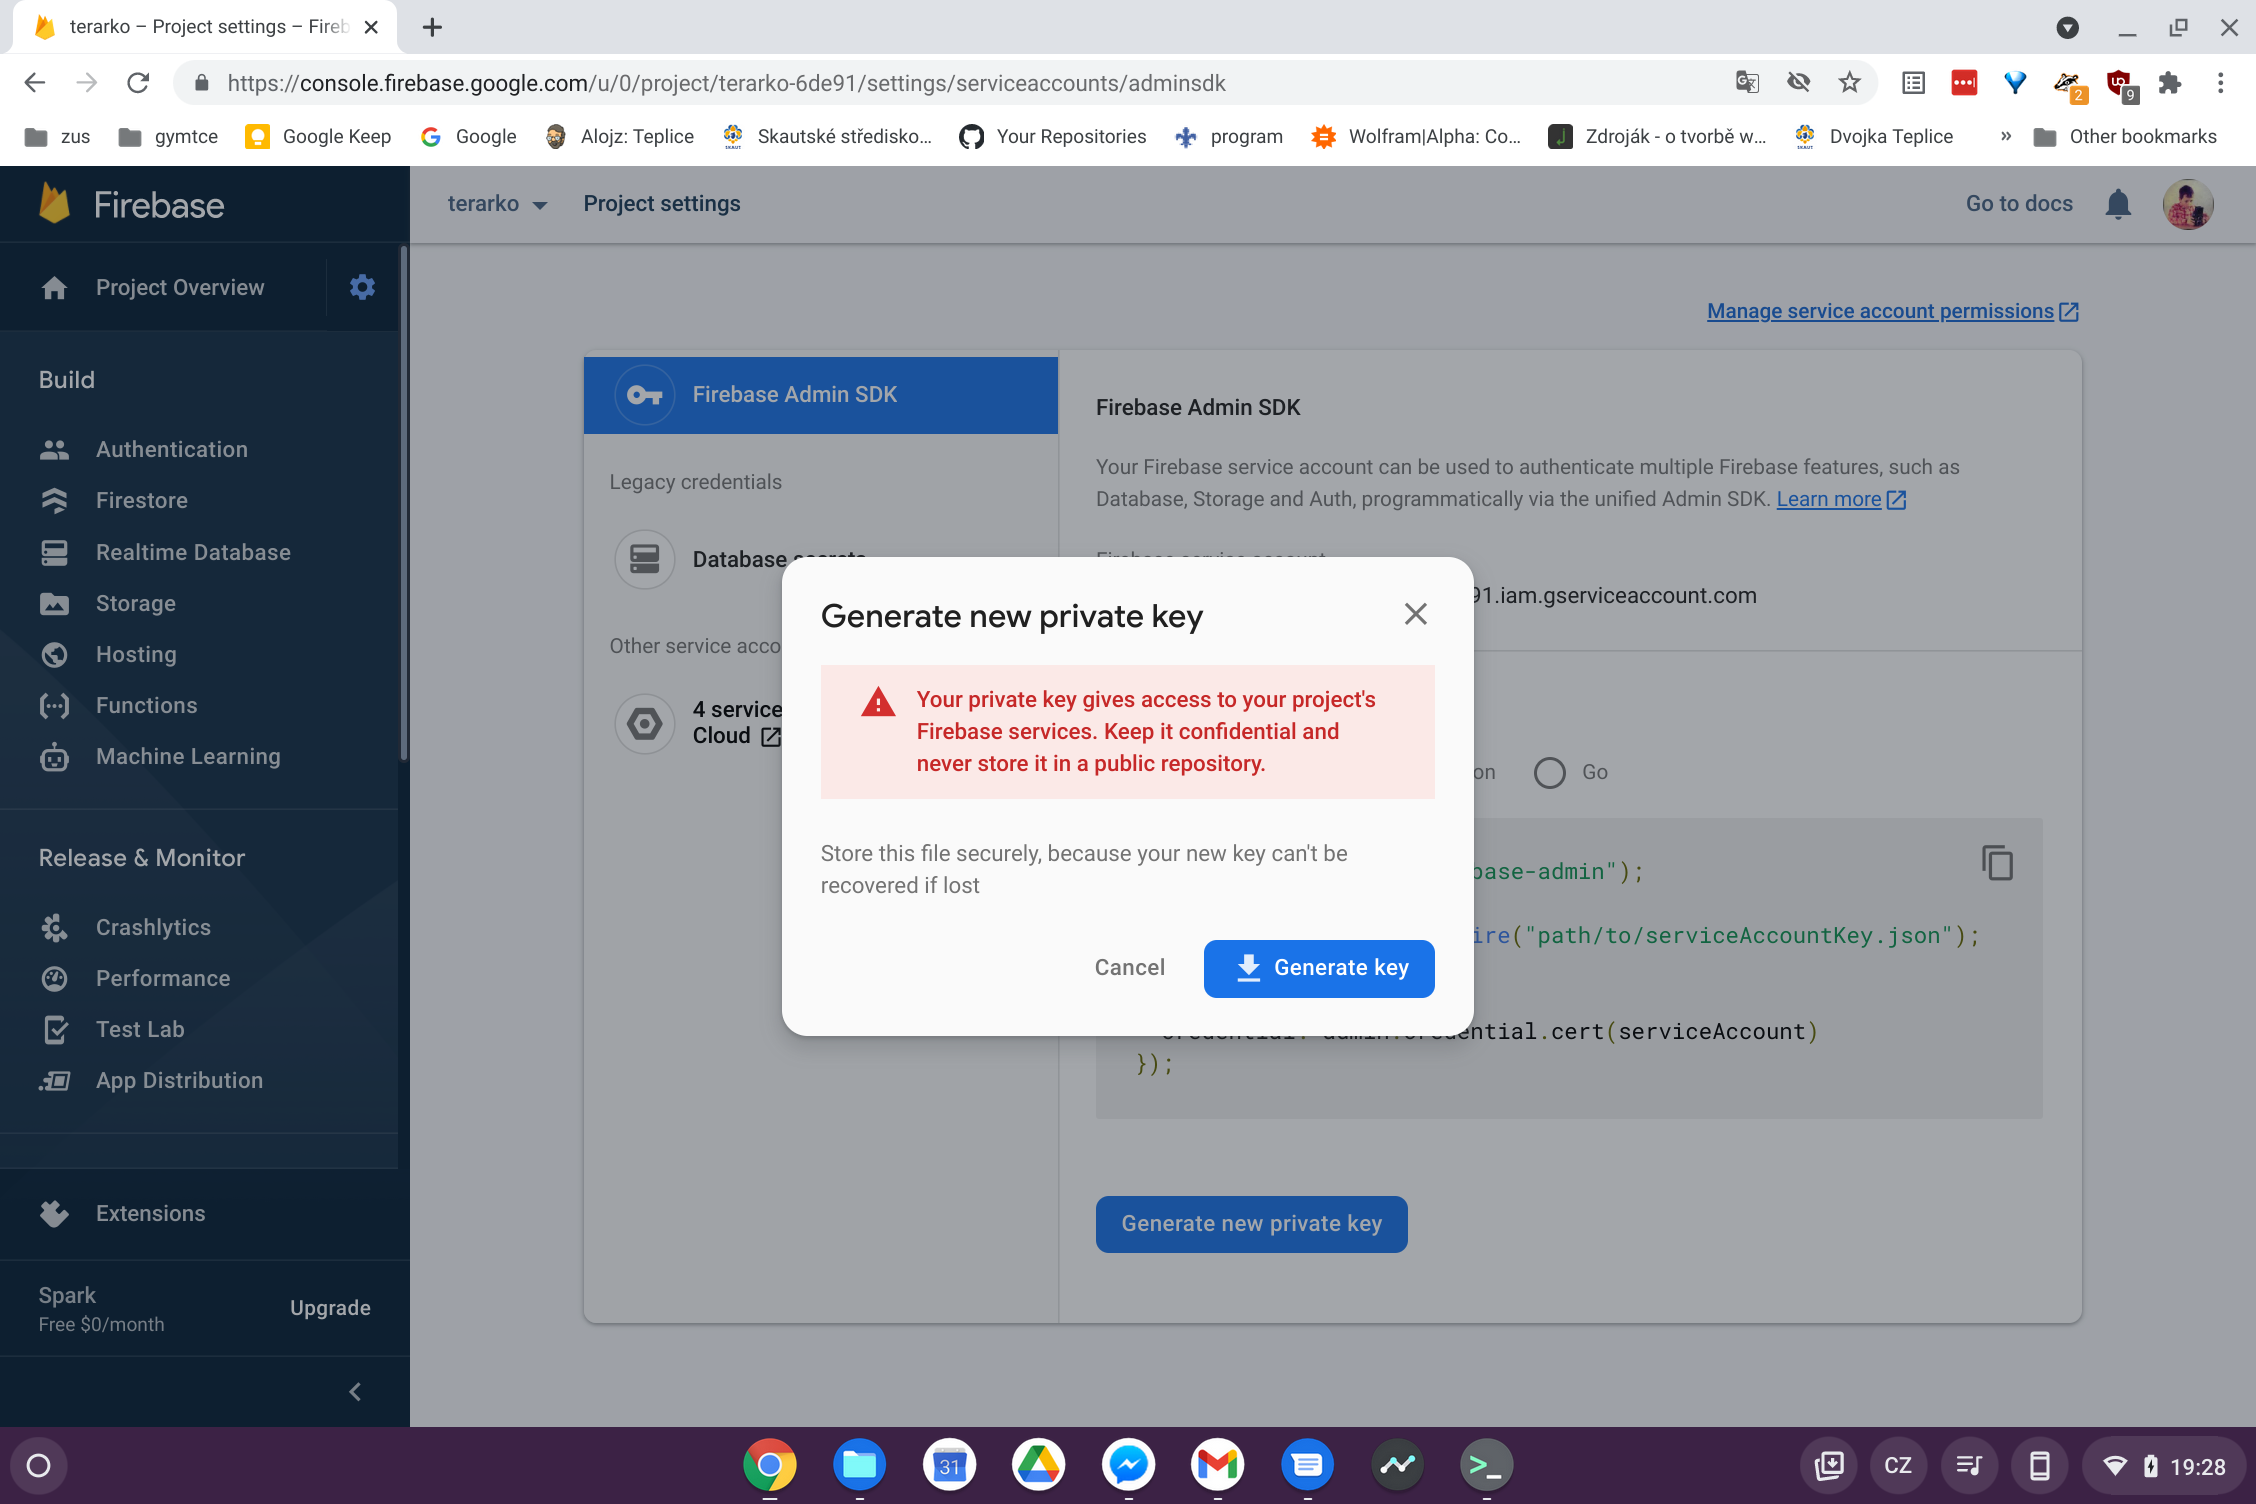
\includegraphics[width=0.8\textwidth]{key2.png}
    \caption{Vygenerování klíče, krok 2}
\end{figure}

\paragraph*{Organizace dat}
Pro každý senzor mám v databázi samostatnou kolekci, ve které je jedno měření představováno souborem, jenž obsahuje 
naměřená data a \gls{timestamp}. Název souboru nechávám generovat firestore, pro mě je nepodstatný.
